\documentclass[10pt]{article}

\usepackage[margin=1in]{geometry}
\usepackage{stfloats}
\usepackage{url}
\usepackage{caption}
\usepackage{subcaption}
\twocolumn
\usepackage{graphicx}
\usepackage[superscript,biblabel]{cite}

\flushbottom

\author{Daniel Speyer\\dls2192@columbia.edu \and Johan Mena\\j.mena@columbia.edu}
\title{\textbf{A Recursive Systemic Profiler}}
\date{}

\usepackage{array}
\newcolumntype{C}[1]{>{\centering\let\newline\\\arraybackslash\hspace{0pt}}m{#1}}

\begin{document}

\maketitle

\begin{abstract}

Understanding how processes spend their time is no easy task: as systems
increase their size and interact with other processes, it becomes more
challenging to track them down. Gathering data is thus of crucial
importance---the more of it there is, the bigger the potential to make better
decisions.  This translates into performance optimizations, bug squashing, and
even addressing issues that were previously unknown. The standard tools for
gathering data about processes are profilers, which measure where processes
spend their time while running. However, most profilers measure things like
CPU, memory or system calls independently, but more often than not,
optimizations are a combination of all these metrics. Furthermore,
most profilers either observe a single process or the entire system,
while most tasks of interest involve many -- but not all --
co-operating processes. We propose and implement
a Recursive Systemic Profiler (RSP) a tool that can intelligently interconnect
different metrics and provide visualizations that give programmers a more
complete view of their systems.

\end{abstract}

\section{Introduction}
Even though premature optimization is the root of all evil, profiling the
performance of a system is critical for its improvement. Profiling is, however,
no small task: one has to know exactly where in the operating system to look for
clues about program behavior, pick the appropriate tool out of several to collect
information, and finally make sense of all the data that comes back.

We know from experience that, most of the time, the slowness of systems doesn't
come from the entire system but from very specific parts. As programmers, we want
to be able to identify where exactly these parts are so that we can optimize only
those parts and not waste time optimizing unimportant parts. We have identified
three steps in order to effectively profile programs: reconnaissance, data
collection and data interpretation. We describe each part next.

First, one needs to have an idea about where the slowness of their program is
coming from: is it spending a lot of time doing I/O? Are high levels of
concurrency causing lock contention? Does it depend on an external process to
make progress? Based on the kind of process being analyzed, this task can range
from either being trivial or hard to identify.

Once one knows where the slowness is coming from, the next step is to collect
data. A very typical but rudimentary way to achieve this would be to insert print
statements throughout relevant parts of a program. This would allow us to get a
sense for the parts of the code being executed, and to a limited degree, to see
if our program does what we think it does. However, this is often not reliable,
especially for programs that interact with several other pieces. This is where
profilers come into play. There exist several of them for virtually every part of
Linux systems: some are targeted only at some particular part of the system while
others are more general and offer higher level information.

Finally, once the relevant data has been gathered, one has to interpret it. This
is sometimes not as trivial as it sounds because the data could come from many
sources: the hardware, the kernel, user applications, etc. At first glance, these
sources can be seemingly unrelated, however, when data is  presented by taking
into account the notion of an interconnected system, it could tell an entirely
different story.

We present the Recursive Systemic Profiler (RSP), a tool that makes it easy to
profile and visualize the behavior of programs. RSP is aimed at programmers
wishing to understand how programs spend their time and how they interoperate
with other programs as well as with various parts of the operating system. This
allows programmers to quickly answer questions like: Why is this process slow?
What is it waiting on? How can I improve it?

\section{Motivating Examples}

The guiding principle of RSP is that looking at one process is not
enough. To that end, here are five scenarios in which that is true.

The classic design of a web application has separate processes for web server,
application server and storage backend. Sometimes the web server is divided
into a base server and a cgi script, and sometimes there are multiple storage
backends. Every request therefore touches numerous systems, but a single
engineering team is responsible for end-to-end performance.

Launching any new process in X11 will involve interactions of the process, the
X server, the window manager, and possibly the composition manager. These
interactions can be quite complex. For example, the application may wish to
store its icons in X's memory. This is also a case in which a merely systemic
profiler will fail, as it is inevitable that the X server will do
\emph{unrelated} work while the launch is taking place.

Any distributed database, by nature, will involve a large number of processes.
It is generally possible to run them all on the same host, but getting useful
performance data from several threads simultaneously remains a challenge.

Compilation of any complex project is often frustratingly slow and also
notoriously difficult to profile, owing to the large number of short-lived
processes and the substantial combined amount of time.

Playing video requires the interaction of the video player, X server, window
manager and composition manager as described in the launch case, as well as the
sound system (\begin{tt}pulseaudio\end{tt} and \begin{tt}alsa-sink\end{tt} on
our test system). In addition, the video player interacts directly with the
video card, using hardware-accelerated resizes, subpicture mixes, colorspace
transforms, and in some cases decoding. Performance in video is a
particularly interesting problem as it experiences hard deadlines every 16ms,
and missing a single one produces a user-noticeable glitch.

We'll return to these scenarios when we evaluate our work.

\section{Data Collectors}

\subsection{Overview}

In order to understand how a system is performing, we first need to collect
data. There are several open source profiling tools that focus on this task. We
can classify them in three different groups by the approach they use to collect
information: event-based, sample-based and a combination of both.

Event-based tools work by instrumenting programs: they insert marks at
different points of a system and trigger an event when the profiled application
runs into them. These events can in turn trigger predefined data-collection
actions as simple as incrementing counters, but they can also perform more
complicated tasks like saving stack dumps for later analysis or generating some
kind of logging.

Sample-based tools work by collecting samples of programs every certain number
of ticks, as predefined by the user. Samples can come in the form of
performance counters, stack traces, or something of relevance that is already
available at the operating system level. These kinds of profilers are
typically less accurate than event-based profilers because they rely on
samples, but since they don't introduce the overhead of generating events as
event-based tools do, they are usually less intrusive performance-wise to the
profiled application.

A third approach combines event-based and sample-based profiling. Instead of
collecting samples every certain number of ticks, these profilers get a sample
after a predefined number of occurrences of some event.

\subsection{Current Tools}

There are a variety of open source tools within these categories for collecting
data in Linux-based operating systems. They vary in functionality and mode of
use depending on the part of the operating system the user is interested in
analyzing or the level of data granularity desired. Some examples of these
tools include \begin{tt}perf\end{tt} for system-wide profiling,
\begin{tt}strace\end{tt} for system call profiling or \begin{tt}netstat\end{tt}
for network profiling.

When we started pondering ideas for how to gather data to create RSP, one of
the first questions that arose was the one about data gathering: would we
simply create a custom tool or would we use something that's already available?
After researching the profiling landscape for 5 minutes, we found out that data
collection was a really challenging task, so we decided to piggyback on
something proven and reliable. Since RSP focuses on giving users a full-picture
view of the system, tools such as \begin{tt}strace\end{tt} or
\begin{tt}netstat\end{tt} where out of the question. We mainly explored two
such tools: \begin{tt}perf\end{tt}\cite{perfwiki} and \begin{tt}lttng\end{tt}
\cite{lttng}, which we discuss next.

\begin{figure*}
\begin{minipage}[b]{.3\linewidth}
\centering%
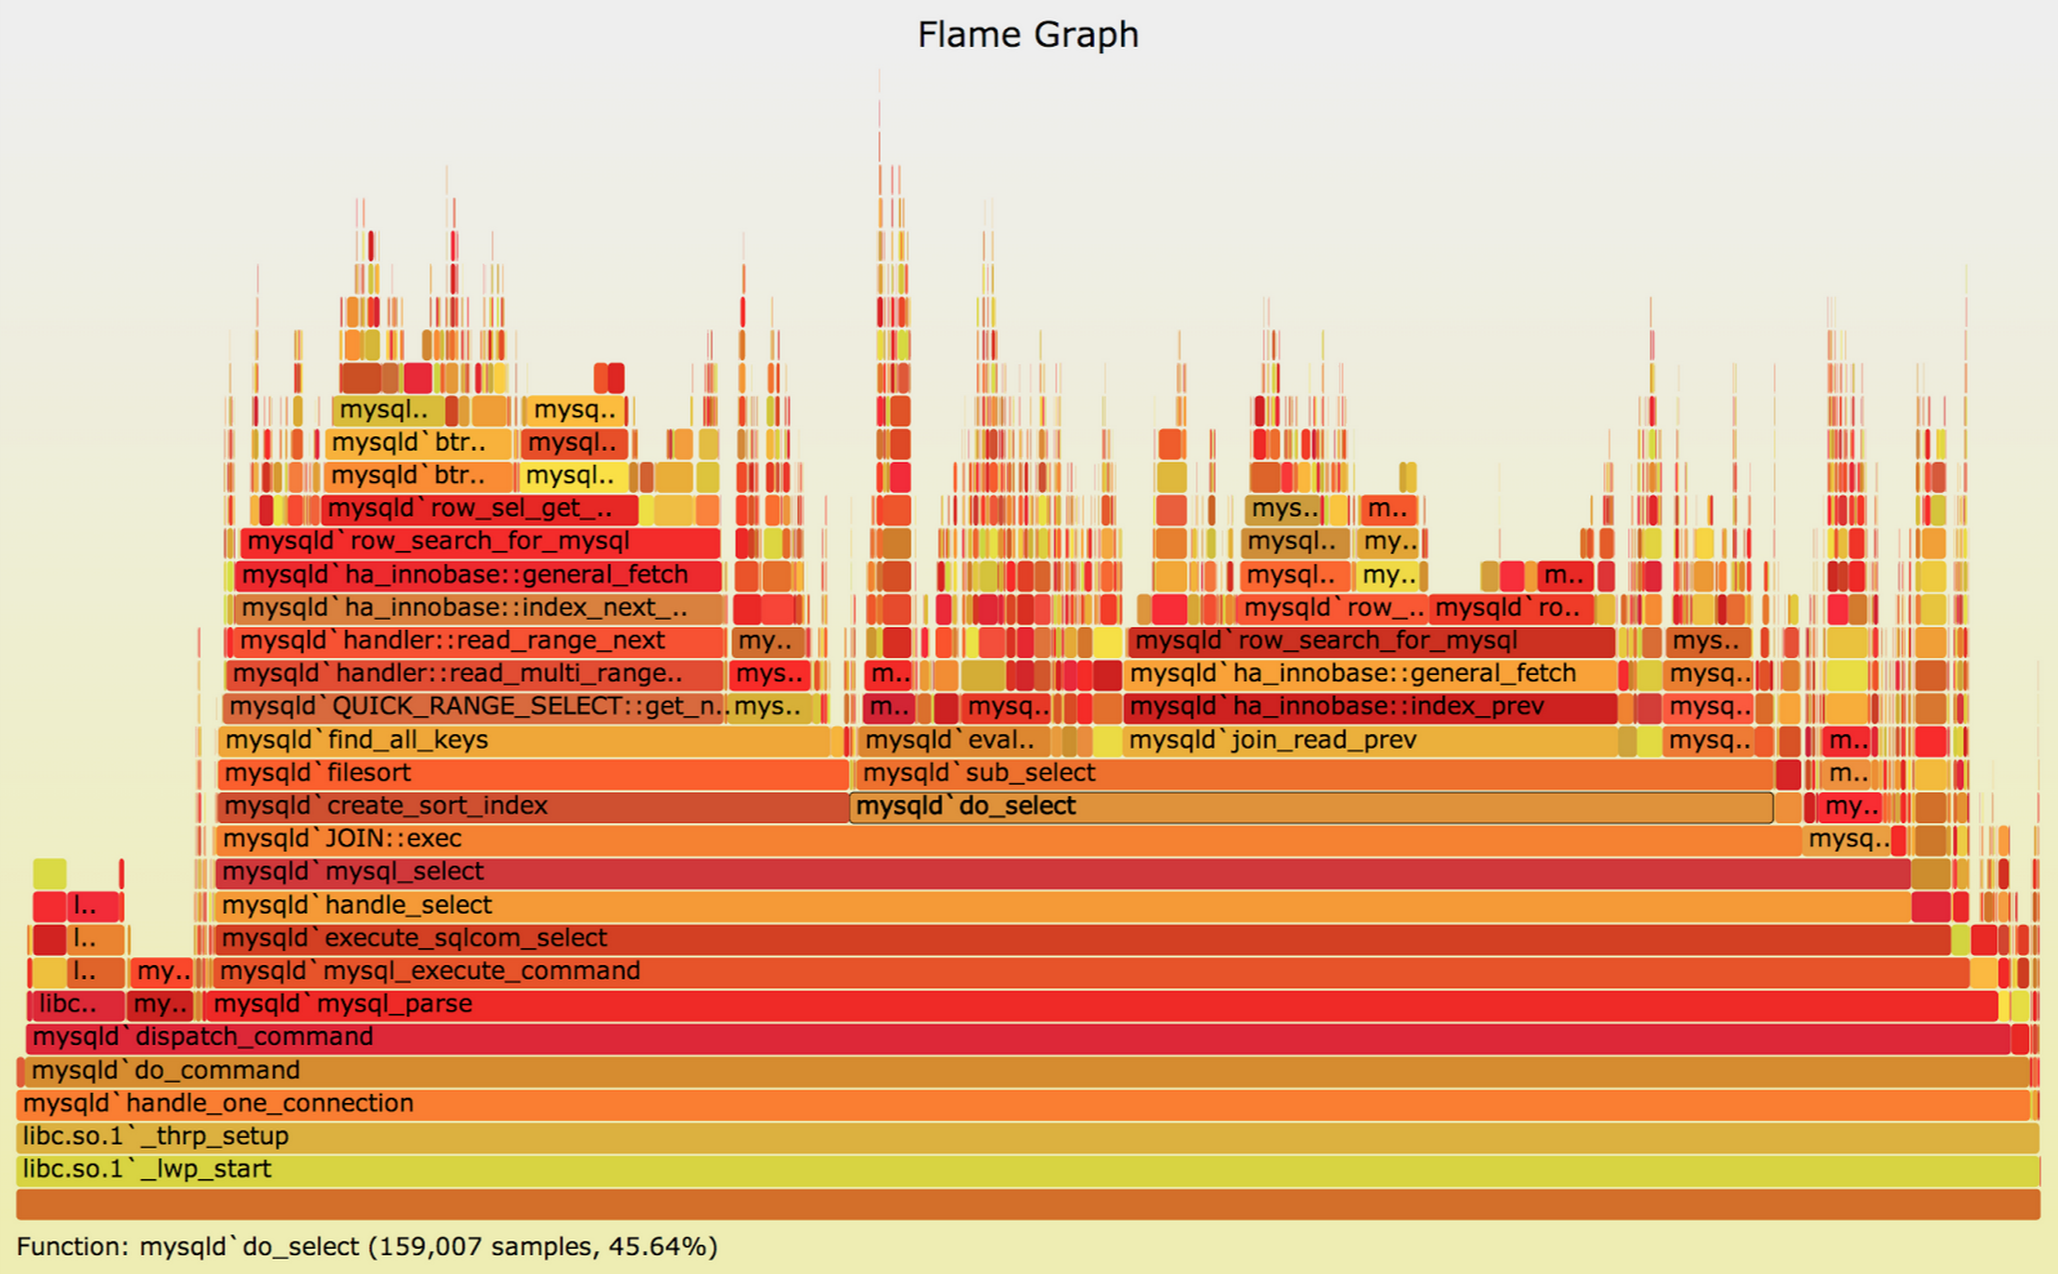
\includegraphics[width=150pt]{images/oncpu}
\subcaption{On-CPU}\label{fig:1a}
\end{minipage}%
\hfill%
\begin{minipage}[b]{.3\linewidth}
\centering%
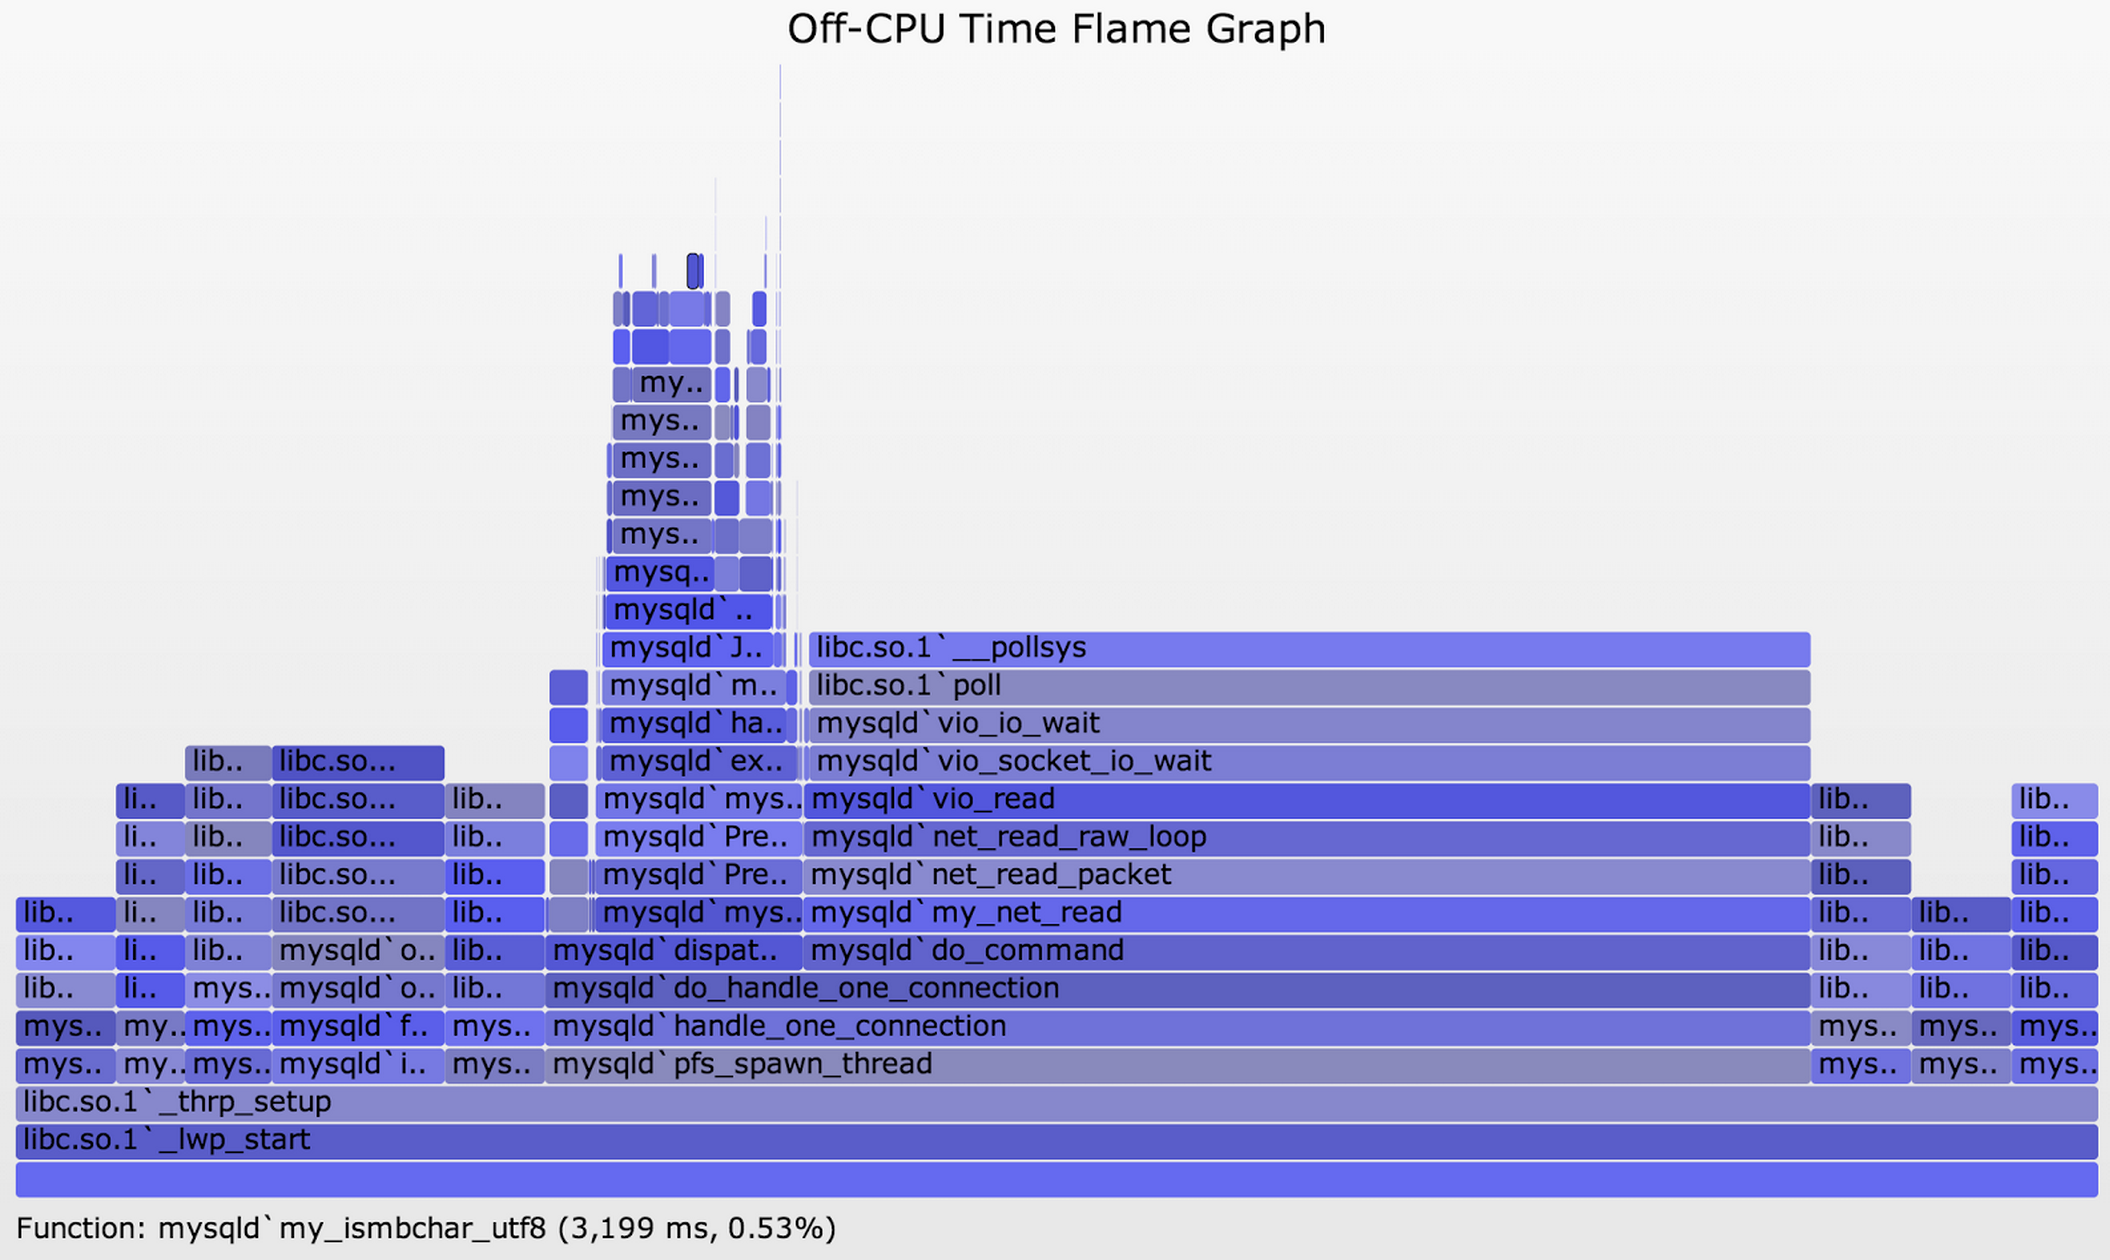
\includegraphics[width=150pt]{images/offcpu}
\subcaption{Off-CPU}\label{fig:1b}
\end{minipage}
\hfill%
\begin{minipage}[b]{.3\linewidth}
\centering%
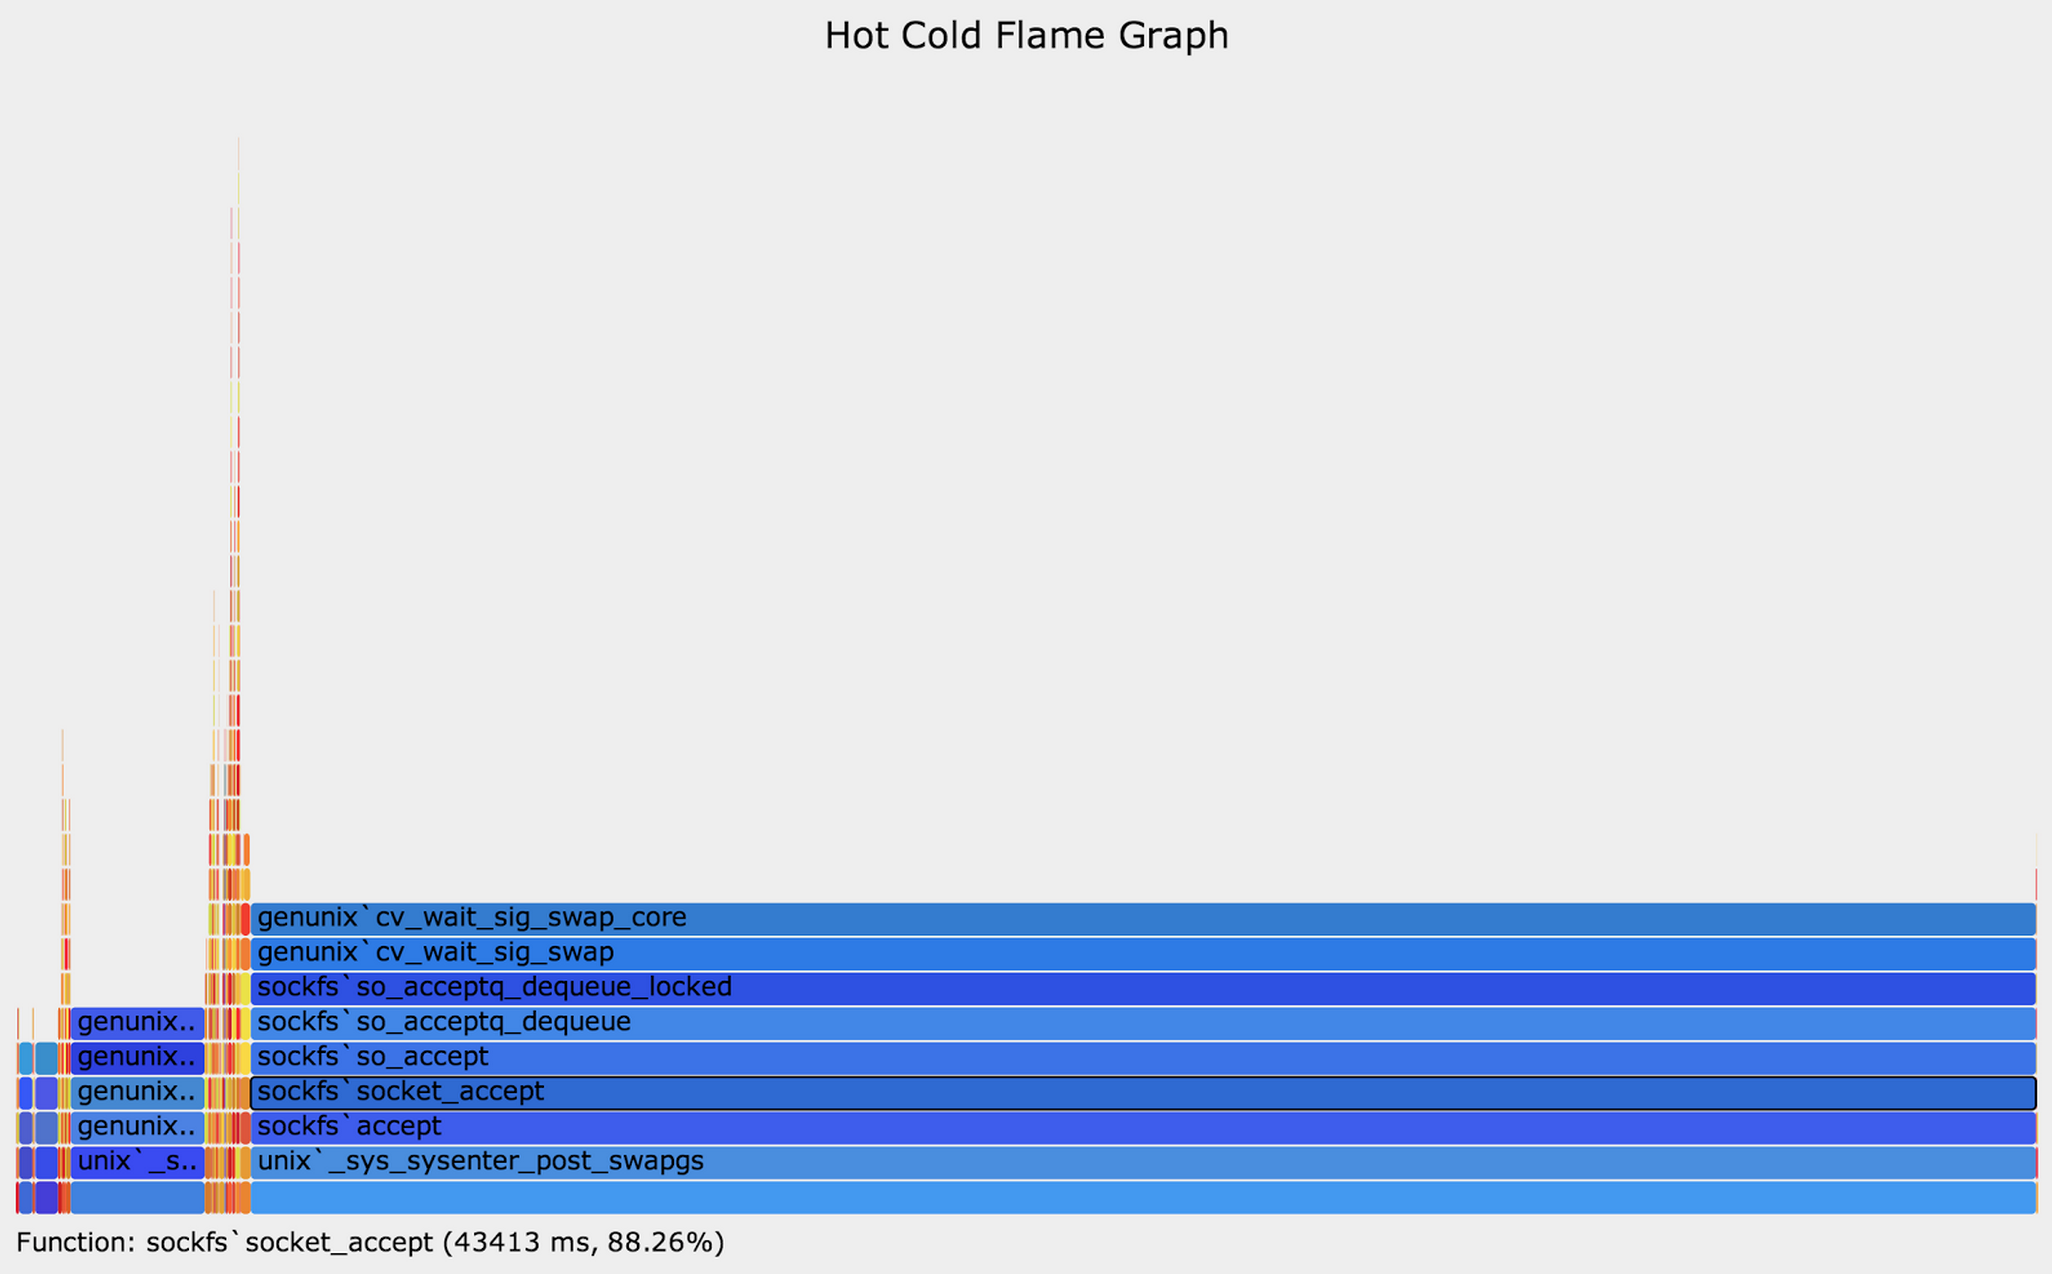
\includegraphics[width=150pt]{images/hotcold}
\subcaption{Hot/Cold}\label{fig:1c}
\end{minipage}
\caption{Flame Graphs}\label{fig:flamegraph}
\end{figure*}

\subsubsection{perf}

\begin{tt}perf\end{tt}, also known as \begin{tt}perf\_events\end{tt} and
\begin{tt}Linux Perf Events\end{tt}, compared to similar tools like ftrace or
\begin{tt}lttng\end{tt}, has the advantage of being a mature and actively
developed tool that can collect system-wide information in a combination of
sample-based and event-based fashion.

\begin{tt}perf\end{tt} can gather per-process performance counters like CPU
cycles and memory cache misses; software events like CPU migrations and minor
faults; as well as high-level behavior like system calls, TCP events, disk and
file system I/O, etc. One can choose which kinds of events to track and
\begin{tt}perf\end{tt} collects statistics on them.

\begin{tt}perf\end{tt} also offers dynamic tracepoints, a feature that taps
directly into symbols and registers when there is no debug information
available and into function names and line numbers when there is.

In addition to these characteristics,\begin{tt}perf\end{tt} is part of the
Linux kernel itself, so not extra dependencies are needed in order to start
profiling Linux applications.

\subsubsection{lttng}

Another system-wide data collection tool that caught our attention was
\begin{tt}lttng\end{tt}. Even though \begin{tt}lttng\end{tt} is not as mature
as \begin{tt}perf\end{tt} is, it offers features such as multiple simultaneous
traces and a \emph{flight recorder} mode\cite{lttngLwn}, in which data can be
collected and analyzed in real-time.

Much like \begin{tt}perf\end{tt}, \begin{tt}lttng\end{tt} can perform combined
tracing of both kernel and user space processes to allow users to monitor
tracepoints, CPU counters, functions and offers the ability to define
dynamic tracepoints when those are not enough.

Unlike \begin{tt}perf\end{tt}, however \begin{tt}lttng\end{tt} is not Linux
kernel specific, and it provides what it calls a Common Trace Format (CTF),
a format of data output that is Linux independent and that according to its
designers, was designed to be streamed over the network for real time
analysis.

Finally, Since \begin{tt}lttng\end{tt} is not in the kernel, it requires the
installation of separate packages.

\subsubsection{Our choice}

We decided to only target the Linux kernel with RSP since that is what we are
familiar with. We felt \begin{tt}perf\end{tt} contained all the features we
needed in this regard, the most important being its ability to
seamlessly gather kernel-space and user-space stacks without any extra
instrumentation (as is the case with \begin{tt}lttng\end{tt}).

Another major point for \begin{tt}perf\end{tt} is that, thanks to being the
ubiqutuous tool for Linux profiling, it contains vast amounts of
documentation that we found invaluable.

\section{Data Visualizers}

Visualizations are at the heart of the Recursive Systemic Profiler. Not only do
visualizations help us understand what's happening in a system in a shorter
period of time compared to reading plain text output, but they also show at-a
glance information that can easily be overlooked when analyzing raw perf or lttng
stack and event traces.

\subsection{Current Tools}

There are a few data visualization tools currently available, both commercial and
non-commercial. We focus on the non-commercial options since they're the ones we
can afford. In particular, we explore two different tools. The first one is Flame
Graphs, which is a direct translation of raw perf output, and the
second one is TraceCompass, a more robust, full-fledged Java application for
visualizing lttng data.

\subsubsection{Flame Graphs}

Flame Graphs, a visualization tool invented by Brendan
Gregg\cite{brendanGregg}, are a simple way to visualize profile data through
stack traces. Stack traces contain the names of the functions being executed by
the CPU at any given time. The information that the stack traces contain can
vary depending on the kinds of process being analyzed, the events one requests
to be notified of, or the duration of the profiling.

One of the key characteristics of flame graphs is that they present their
information in a hierarchical, stack-like manner, in such a way that one can
easily tell which stacks frames were triggered by which other stacks frames,
making it easy to see what's going on once one gets accustomed to the format.

Flame graphs also have the characteristic of being able to show at a glance
overall slow hot-spots (represented by the width of the function calls in the
stacks) and overall program structure.

We drew our attention to three kinds of Flame Graphs: On-CPU\cite{oncpu},
Off-CPU\cite{offcpu} and Hot/Cold Graphs\cite{hotcold}.
Figure~\ref{fig:flamegraph} shows examples of these three kind of flame graphs.

On-CPU flame graphs are the ones that show a process and its threads spending
time running on CPU.

Conversely, Off-CPU flame graphs are the ones that show how a process waits.
However, these kinds of graphs can be a little difficult to interpret, as they
require tracing and interpretation of wake up events.

The combination of those two is what's known as a Hot/Cold flame graph. This
shows a more complete view because it displays what was happening at the time
when the process was running as well as when it was waiting. Despite this, the
combination of on and off CPU flame graphs can confusing to interpret because
the sum of all threads sleeping is usually a lot bigger than the time spent
doing work, therefore, as Figure~\ref{fig:1c}, the On-CPU part can get very
narrow---but this could probably be addressed with zooming capabilities (which
is the approach RSP takes).

\subsubsection{TraceCompass}

\begin{figure}[h]
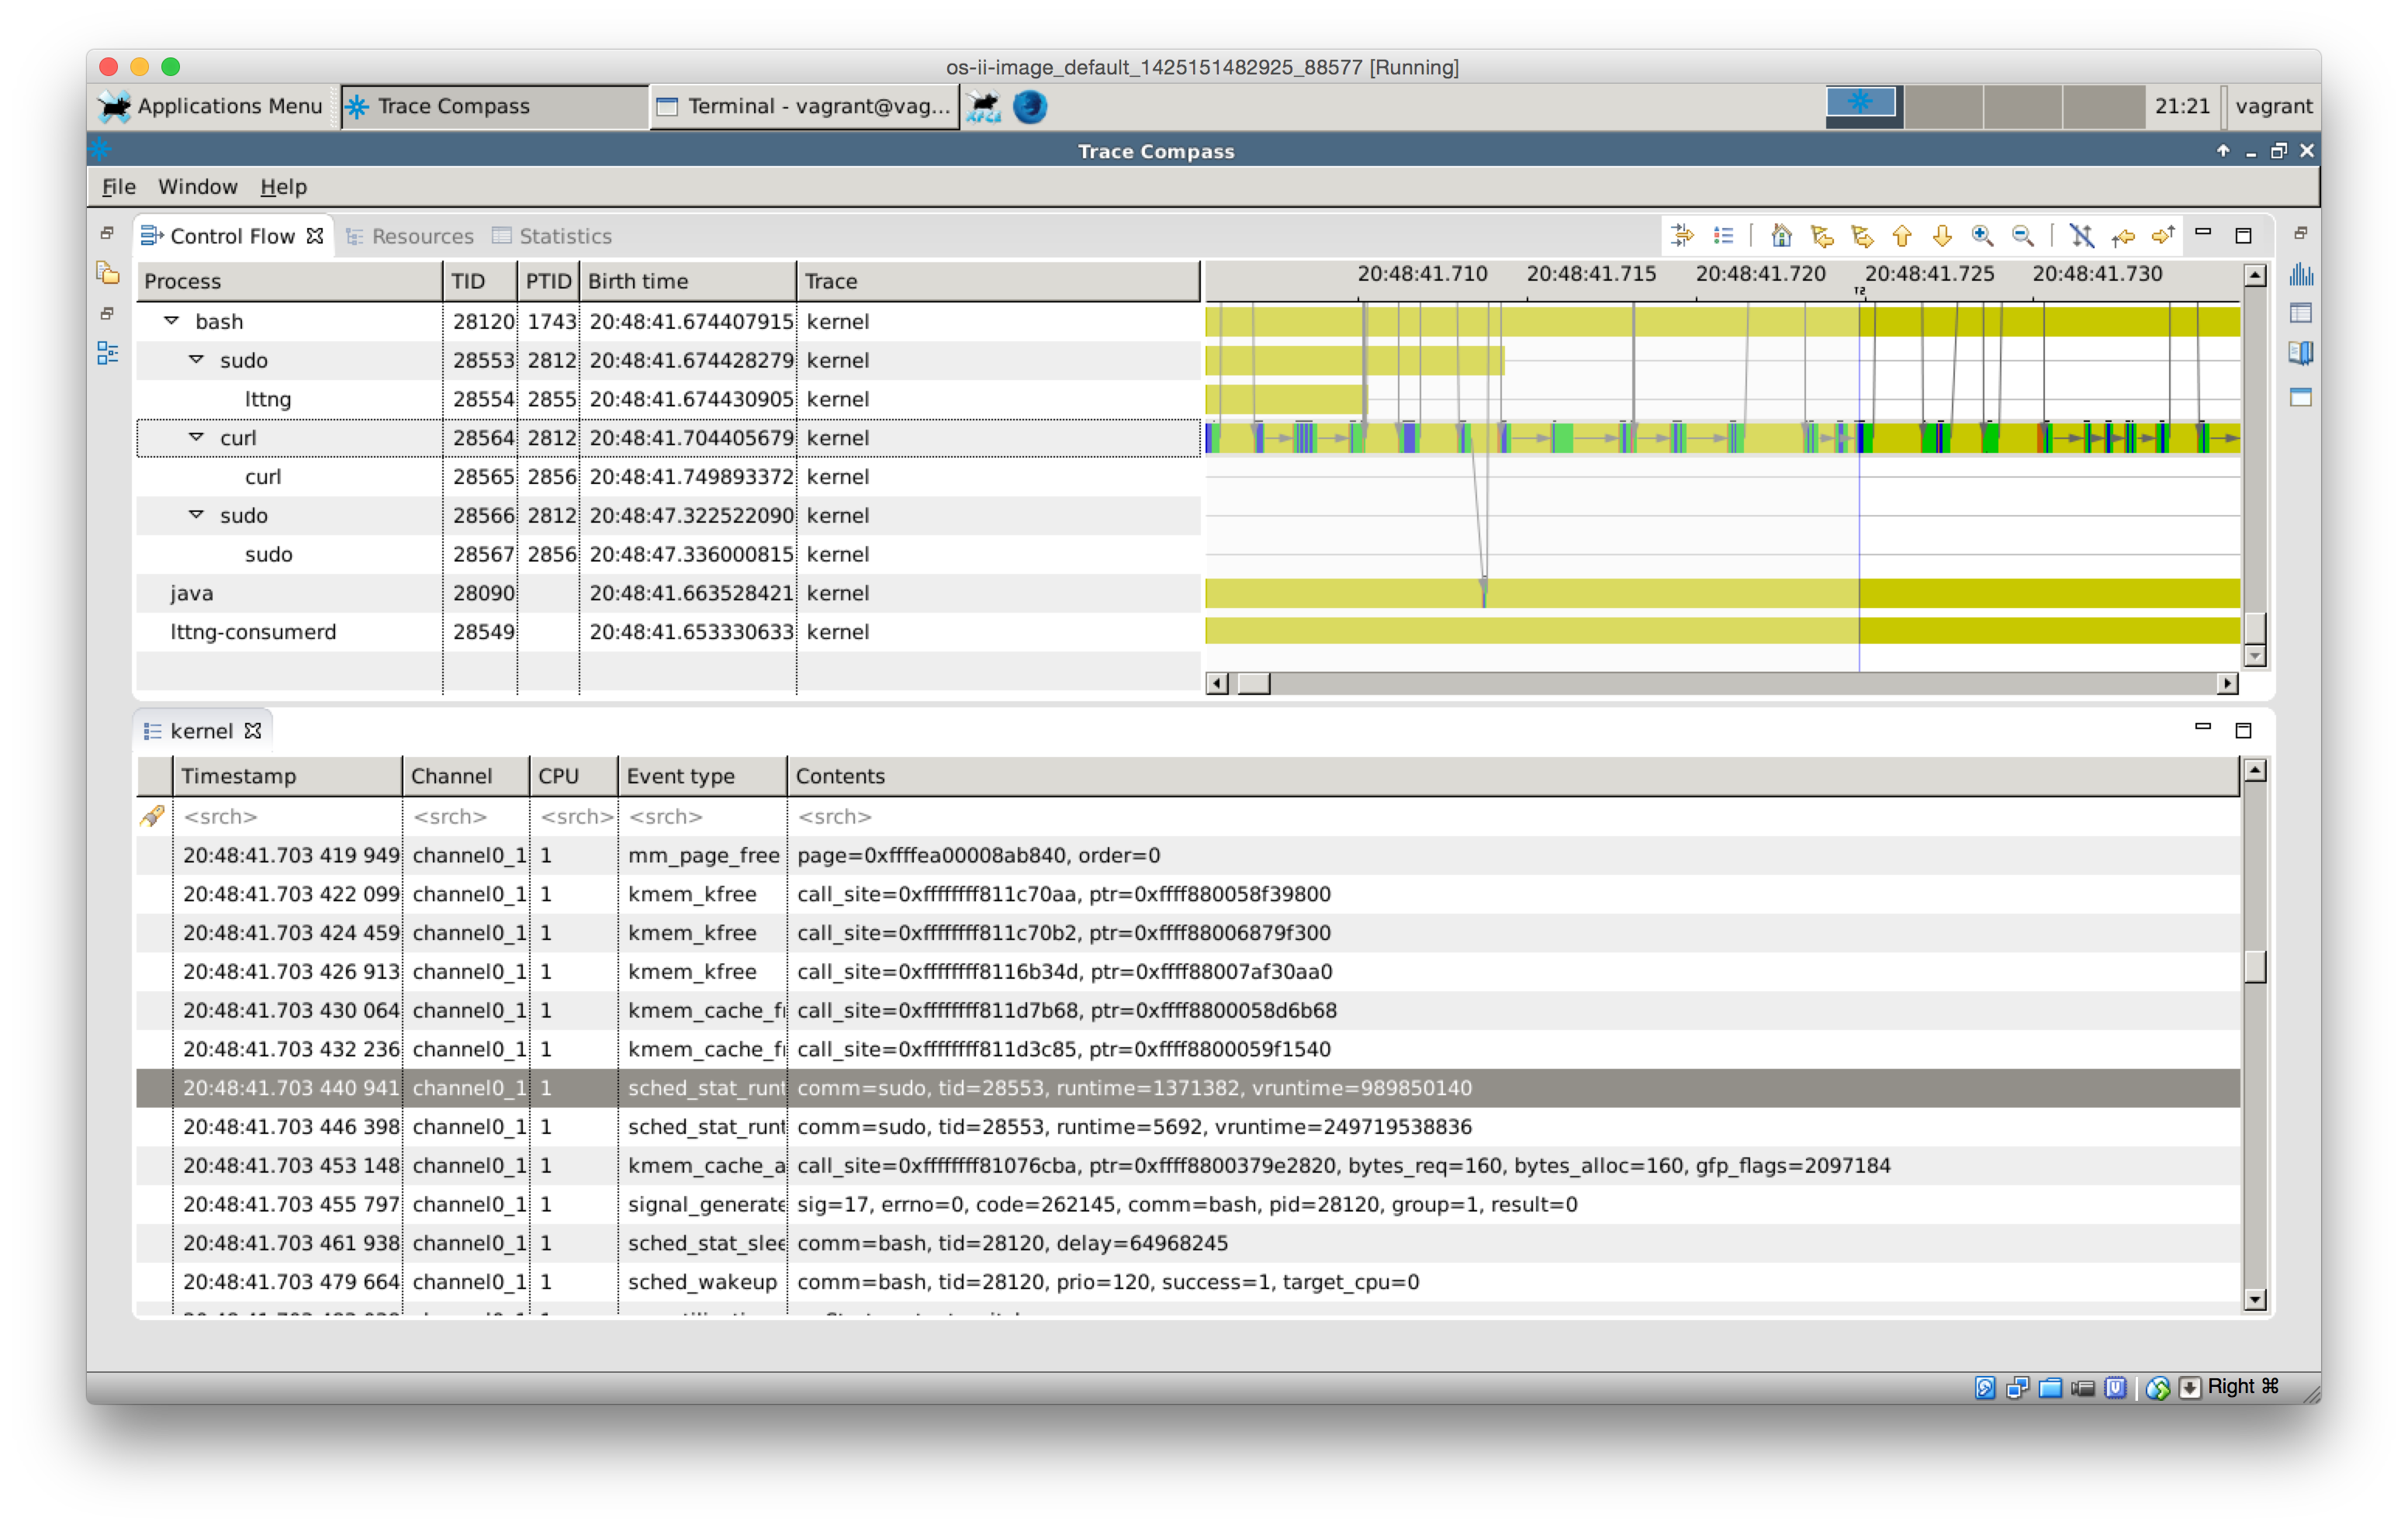
\includegraphics[width=3.25in]{images/tracecompass}
\caption{TraceCompass}
\label{fig:traceCompass}
\end{figure}

TraceCompass\cite{traceCompass} is a Java tool that uses lttng as its data
collector and leverages the Eclipse framework to create a full-fledged data
visualizer. Once lttng data has been collected, one can start visualizing it in
an interactive manner.

It is worth nothing that TraceCompass offers some a dizzying array of options
and functionalities. But for the sake of our research, we focus on what makes
it similar to RSP (which turns out to be the core of the program).

Figure~\ref{fig:traceCompass} shows TraceCompass' three main components: A
Control Flow window (top left) presented in a collapsable tree structure that
makes it easy to see parent-child relationships that were part of the trace. A
Visualization window (top right), which is attached to the Control Flow window
and where one can visualize processes (represented as blocks whose length are a
function of the time the process ran) and their transitions. And a scrollable
Events window (bottom), where all raw event samples are displayed in a
chronological order using a tabular format that is filterable on columns like
the timestamp, the event name or the contents (like function arguments or
return values in the case of a system call) of the event that were recorded.

In addition to this, TraceCompass also offers a statistics view for seeing the
counters or percentage distribution of various events that happened during trace.

TraceCompass suffers from the drawbacks of other visualizers. First, it is not
able to smartly connect data very well. For example, if a process gets blocked
on a mutex, that process and the provider of the mutex won’t be connected.
Second, since application stack frames are not present in the visualization
itself, it is rather hard to interpret, as one has to go back and forth between
the three windows to make sense of the information. Finally, since events in
the Events window are laid out in a simple chronological manner, it is not easy
to make sense of processes with high degrees of parallelism because other
events interfere.

\section{Recursive Systemic Profiler}

The Recursive Systemic Profiler is designed to measure all the activities that contribute to the running time of a program.  It is ``systemic'' in that it records everything that takes place on the system and ``recursive'' in that it starts from a process of interest, then considers processes that was waiting for, and processes those were waiting for, and so on.

The building blocks the profiler works with are runs, sleeps, links and samples.  A run is a contiguous block of time during which a process is running.  A sleep is a similar block in which the process is not running.  A link marks one run causing another.  And a sample is taken by the sampling profiler.  Each sample is part of a run, but very short runs may not have any samples.

\subsection{Pseudo-stacks and Control Paths}

A set of connected runs with negligible overlap can be called a ``control path''.  Conceptually, this is a single series of tasks.

One common pattern is for one process to transfer control to another, and then the other to transfer control back.  Both transfers could be tcp messages, as in the case of making a synchronous rpc request to a database, or one could be a \begin{tt}fork\end{tt} syscall and the other a \begin{tt}wait\end{tt} syscall terminated by the other's exit.  In these cases, it is fairly reasonable to think of the first transfer as a ``function call'' and the second as a ``return''.

While not every pattern of process interaction naturally fits this view, those which don't can generally be shoehorned to fit with fairly little damage.  For example, if one process wakes another which wakes a third which wakes the original, we can think of the first as having been a child of the second, even thought the call went directly.

Once we have this concept of calls and returns, we can assemble the processes into something like a stack.  Note that only the top element of the stack will be a run -- all the rest will be sleeps.

\subsection{Visualizations}

Once we have our data gathered, the next task is to visualize it.  We have three views to do this with.

Our examples here use a toy program called ``pass''.  Pass forks two processes, connects them with pipes, and then runs in a loop in which one process does some work, then writes to one pipe (waking the other process) and reads from the other pipe (blocking on the other process).  It is called ``pass'' because it passes the act of doing work back and forth.

\subsubsection{Process Running View}

The first view is the Process Running View.  It uses an x axis of time and a y axis of processes.  Each run is a block bar, and each link is drawn as a line between them.

\begin{figure}[h!]
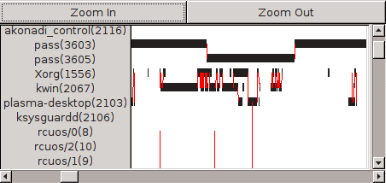
\includegraphics[width=3.2in]{images/screenshot}
\caption{The Process Running View}
\end{figure}

The view also contains an option to show sleeps, which are drawn as blue boxes.  Sleeps are labeled with one function from the stack which best describes the sleep.  At the moment, this is the innermost userspace function, which roughly corresponds to the blocking syscall as the programmer would conceive of it.

Clicking on a process name opens a Flame View for that process.

\subsubsection{Flame View}

The Flame View takes a single process and shows all associated processes, organized into control paths.  Each control path is treated as a series of pseudostacks, and each layer of each pseudostack is drawn as its stack.  This presents the concept of a single stack of functions stretching across multiple processes, which is a pretty good fit for how many programs are actually designed.

\begin{figure}[h!]
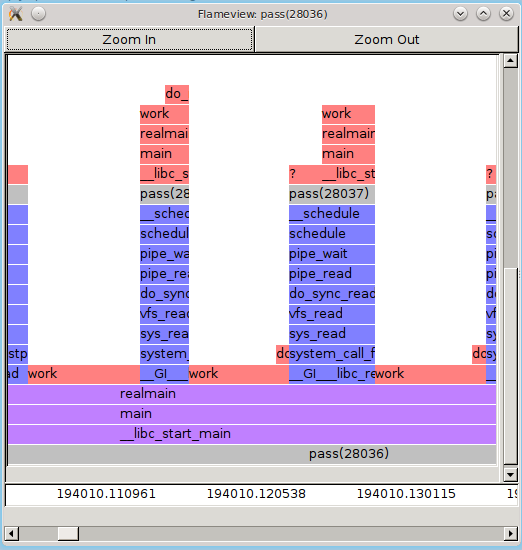
\includegraphics[width=3.2in]{images/flameshot}
\caption{The Chronological Flame View}
\end{figure}

Functions in a run stack are shown in red, whereas those in a sleep stack are shown in blue.  Functions in both (i.e. those which call both sleep and run subroutines) are shown in purple. Process names are shown in grey.  Blocking IOs (not in this example) are green.  Links are still shown, though links within a control process tend to be largely invisible.

If a run has multiple samples, the horizontal space of the run is divided equally.

The x axis is still time, but now the y axis is stack depth.

\subsubsection{Consolidated Flame View}

The consolidated flame view is similar to the original flame view, except that all matching pseudostacks are gathered together and then sorted by duration.  More specifically, the bottommost stack frames are sorted by duration, then for each of those the next frames up are sorted and so on.  It provides a nicely compact summary of all the time spent by the process.

Because children are allowed to overlap their parents slightly, the higher stack frames can be significantly longer than the lower ones.  Lower ones are spaced apart as needed to allow for this.

\begin{figure}[h!]
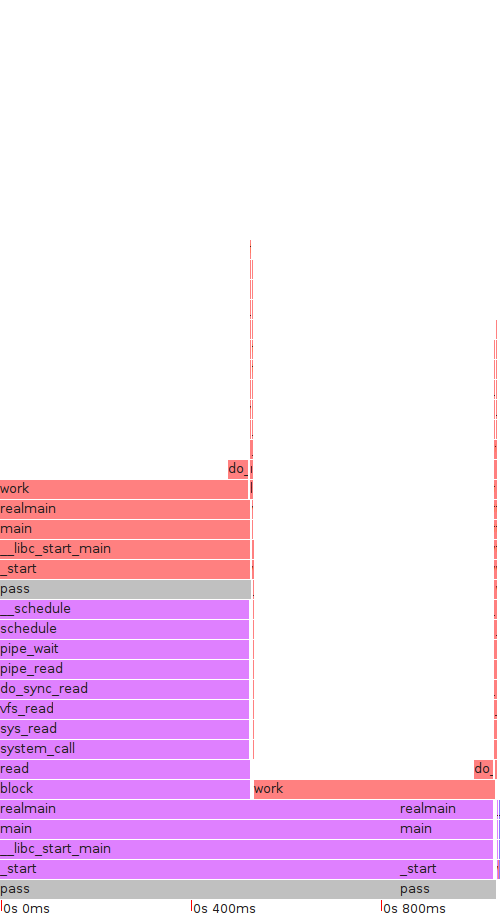
\includegraphics[width=3.2in]{images/passcons}
\caption{The Consolidated Flame View}
\end{figure}

\section{Implementation}

The overall data flow for our tool is simple: gather data with perf record, dump it in textual format with perf script, then interpret it with python and display it with gtk.

\subsection{Obtaining Information}

All our information ultimately begins with perf.

\subsubsection{Ordinary Events}

We monitor eight ordinary events: four from the sched\-uling system, three from the block I/O system, and one from the irq handling system.  These are described in detail in the Assembling Pieces section, along with how they are used.

\subsubsection{Probes}

While Linux does offer events for networking, they are inadequate for our purposes for two reasons.  First, they provide no mechanism for connecting related events.  Also, the ``receive'' events are fired when a process reads data, not when a network operation completes.  Fortunately, perf offers ``probes'', which allow us to select any (non-inlined) kernel function and place an event there with any or all of the function arguments as attributes.

We insert 3 pairs of probes, for the transmission and response of tcp handshakes, tcp content and udp content.  All the probes capture the memory address of the kernel data structures for the socket, which allows us to identify matching operations.  In theory, it should be possible to match this to a remote IP and port pair by inserting an additional probe into the connect call, but this didn't work, probably because of compiler optimizations in the kernel.  

Matching events by socket makes our network support limited to tcp and udp.  A program that blocked on icmp shows itself as ``waiting for hardware,'' specifically the network interface card.  Fortunately the two supported protocols account for the vast majority of internet traffic, and adding others would be fairly straightforward.

The response events attach not to the read syscalls, but to the kernel routines that take network data and turn it into a packet for a specific socket.  This gives us the exact time of the response, and fits nicely with the concept of threads being woken up.

\subsubsection{Stacks}

Perf has native stackwalking support built into the event structure.  It crosses the kernelspace/userspace boundary with no difficulty.  It does, however, fail against frame pointer optimization.  While it is sometimes practical to recompile code without it, recompiling the entire system is not.  As an alternative, perf offers libunwind, also known as ``dwarf'', which uses a variety of heuristics to find parent frames.  This is more reliable, but still cannot trace all stacks.  Another solution is in the works based on the Last Branch Record register of the Haswell microarchitecture, but that is hardware-specific and not yet merged into the mainline kernel.\cite{lbr}

We found a less elegant workaround for the most common cases.

\subsubsection{Userspace Probes}

Perf has the ability to place probes in userspace code as well as kernel.  We identified a small number of syscalls in libc that consistently broke stacktracing and placed userspace probes there.  Since the use of the frame pointer to store data occurred in the middle of the function and the tracepoint at the beginning, we got intact stacks for these tracepoints.  When a process fires a \begin{tt}probe\_libc:poll\end{tt} event with a stack going back to \begin{tt}\_\_libc\_start\_main\end{tt} and immediately follows it with a \begin{tt}sched:sched\_switch\end{tt} event with a stack going back to \begin{tt}poll\end{tt}, we can append the stacks and have a complete stack for the latter event.

As an added complication, perf refuses to create userspace events for ``weak'' symbols, which includes \begin{tt}poll\end{tt} in libc.  This check can simply be removed from perf with no harmful effects, and does not require recompiling the actual kernel.  Why perf has this limit, and why such a common syscall is a weak symbol, remain unclear.

\subsection{Assembling Pieces}

Once we have a stream of relevant events with sufficient attributes and stacks, the next step is to assemble them into a set of ``operations'' and links between them.  An operation is a generic concept useful to visualization: a thing which can reasonably be drawn as a single rectangle.  It can be anything with a beginning, an end, and a single nature.

\subsubsection{Runs and Sleeps}

The simplest operations are ``runs'' and ``sleeps'', which represent contiguous blocks of time in which a given process was either running or not running.  Every \begin{tt}sched:sched\_switch\end{tt} event ends one process's run and begins its sleep, while doing the opposite for another process.  Similarly, \begin{tt}sched:sched\_process\_exec\end{tt} ends one process's run and begins another's, with no sleeps involved (the two processes have the same PID, but we track them as separate.

When a \begin{tt}cycles\end{tt} events (from the sampling profiler) is encountered, we check if the process it shows is running or was in the past $20 \mu$s.  If so, we attach it to that run.  If not, we drop it with a warning.  Why \begin{tt}cycles\end{tt} events continue to arrive for a process so long after it has switched remains unclear, but it is a common occurrence.  Presumably some aspect of the sampler runs asynchronously.

When a \begin{tt}sched:sched\_wakeup\end{tt} event is encountered, if it does not fit any of the special cases below, a link is generated from the run it is inside of to the next run of the process awoken.  When a \begin{tt}sched:sched\_process\_\\*fork\end{tt} event is encountered, a similar link is generated (with no special cases).

\subsubsection{Disk IO}

The lifecycle of a disk IO operation contains four events.  First, the operation is created and placed in a queue.  For this, a \begin{tt}block:block\_rq\_insert\end{tt} is fired from the process that issued the request.  Then, the operation is removed from the queue and send to the device, with a \begin{tt}block:block\_rq\_issue\end{tt} event.  The device can have two operations acting at once, and timing suggests they actually run in parallel, strange as this sounds for magnetic disks.  Finally, the operation completes with a \begin{tt}block:block\_rq\_complete\end{tt} event, and the issuing process is woken up, producing a separate \begin{tt}sched:sched\_wakeup\end{tt} event.  The three \begin{tt}block:\end{tt} events all include the device numbers and the block offset, allowing us to connect them.

The final wakeup event can be recognized by the function \begin{tt}bio\_endio\end{tt} on the stack.  It does not contain the device number of block offset, but it does contain the process to be awoken.  We find the most recently finished block I/O that was originally issued by that process.  This heuristic isn't perfect, but it seems to work for all our test cases.

Sometimes the \begin{tt}block:block\_rq\_issue\end{tt} event is not fired.  When we see an operation that is still in the queue complete, we retroactively assume it was issued immediately after enqueueng.

\subsubsection{Network}

Network operations do not fit perfectly into our model.  A write event followed by a wakeup event produces an operation with links to both runs.  If more read events follow, the operation is regarded as longer, and has multiple outlinks.  Writes which are not followed by reads do not produce operations.  For example, if a browser contructs a very large HTTP request and sends it by multiple \begin{tt}tcp\_sendmsg\end{tt} calls, the loops receiving the response which arrives in several packets, the network operation will stretch from the last write to the last read -- the time for which it is reasonable to say ``the server was doing work that our process could be waiting for''.  Figure \ref{fig:tcp} may make this clearer. 

\begin{figure}[h!]
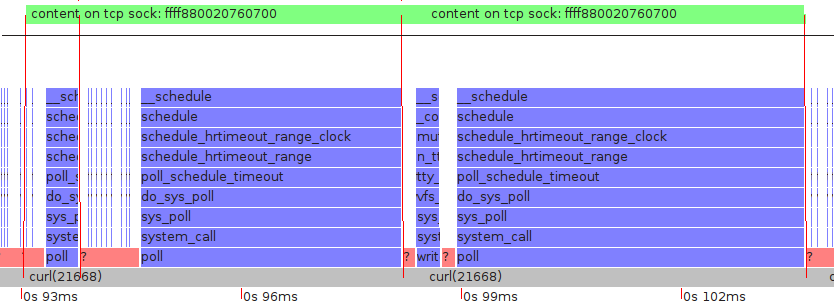
\includegraphics[width=3.2in]{images/tcpexample}
\caption{A TCP operation with multiple wakeups}
\label{fig:tcp}
\end{figure}

In any case, network events are matched by socket address (that's memory address, not IP address) and network wakeups are matched to scheduler wakeups by occuring close in time, in the same process, with the relevant kernel function on the latter stack.

\subsubsection{Interrupts and Preemption}

Wakeup events can be identified as interrupts if the departing stack
contains either the function \begin{tt}do\_IRQ\end{tt} or the
  function \begin{tt}apic\_timer\_interrupt\end{tt}.  For interrupts, we do not make a link between the processes, but instead make a link between the two runs of the interrupted process that have the interrupt in between them.  This link is marked as ``horizontal'', because it does not correspond to a change of stack layer.

\subsubsection{Wakeups}

Links are created not only from wakeup events, but also from fork and exec.

\subsubsection{Recursive Stack Making}

Assembling pseudostacks and control paths is a single procedure.  First, we declare all runs of the process of interest to be in the base control path.  Then for each of them try to make the thing which woke it a child of the sleep that preceded it.  This succeeds if the run starts at most 100$\mu$s before the de facto start of the sleep, and ends at most 100$\mu$s after the sleep ends.  

To compute de facto start times, we consider all consecutive sleeps -- with the same stack, separated by runs of less than 100$\mu$s, such that all but the last end in timeouts -- to be a single sleep.  This handles the common pattern of \begin{tt}while (!done) \{ poll( with timeout ); trivial\_timeout\_processing(); \}\end{tt}.

We allow the child to overlap its parent slightly because this is a very common pattern in multicore environments.

If the child does not fit, we declare it to be of a different control path.  If the original run was of a different control path than the attempted parent, we use that path.  If not, a new one.

We then recurse on both the child and the parent. 

\subsubsection{Triangles}

While a simple stack is the most common pattern, we do see cases of A calls B calls C calls A.  In this case, we treat C as B's parent.  However, C's sleep may begin well before A called B.  If so, only the latter part of C can be described as ``on behalf of'' A.  We cut C there, and do not display the earlier part nor count it for statistics.  Furthermore, we recalculate if C can be on the same control path as A given its new smaller duration.

\subsubsection{Visualizing}

All visualizations are drawn using gtk.

The legend of the main window doubles as launchers for the flameviews (specifying which process is of interest).

Note that sometimes a child will slightly overflow its parent.  This is by design.  So long as the overflow is small, the run is conceptually a child of the sleep, even though it starts first.

In the flamegraphs, adjacent stack elements are unified so long as there is nothing visible between them.  Increasing zoom can cause formerly unified blocks to separate.  This is necessary to fullfill users' expectations for computation-heavy code that suffers from interrupts.

\section{Evalutation}

\begin{figure*}[t]
\begin{tabular}{r|C{.77in}C{.8in}C{.77in}C{.77in}C{.77in}}
Category & Squirrelmail & xterm launch & spatialtable & make & MPlayer\\
Processes & 18 & 13 & 133 & 12 & 17\\
\hline
Wall time & 265 & 315 & 74 & 4438 & 2180\\
Total time & 269 & 603 & 89 & 4712 & 4481\\
\hline
In understood functions & 84 & 86 & 61 & 1526 & 324\\
In blocking I/O & 125 & 0 & 0 & 2845 & 250\\
Running but not sampled & 10 & 66 & 24 & 77 & 130\\
I/O queue overhead & 49 & 0 & 0 & 47 & 0.41\\
Scheduler overhead & 0.96 & 3.2 & 4.6 & 21 & 29\\
Waits ``for'' hardware & 0 & 0 & 0 & 0 & 16\\
Involuntary sleeps & 0.18 & 0.23 & 0.09 & 4.0 & 10\\
Miscellaneous kernel blocks & 0.05 & 0.64 & 0 & 0.26 & 0\\
Waits that timed out & 0 & 226 & 0 & 0 & 3568\\
Waiting on other path & 0 & 191 & 0 & 7 & 10\\
\hline
Total Accounted & 268 & 573 & 89 & 4526 & 4339\\
Unaccounted & 1.2 & 29 & 0.28 & 185 & 142\\
Percent Accounted & 99.6\% & 95.2\% & 99.7\% & 96.1\% & 96.8\%\\
\end{tabular}
\caption{Categories of Explanation for Various Tasks; All times in Milliseconds}
\label{fig:restab}
\end{figure*}

The ultimate test of a performance tool is how much it can explain.  We calculated the total time spent, including all parallelism and broke time we understood into categories which we sorted from best-understood to least-understood.  We offer this data both as a table (\ref{fig:restab}) and as a graph of cumulative percentages (\ref{fig:resgraph}).

\subsection{Test Cases}

We have five test cases, inspired by the five motivating examples from the beginning of the paper.

\subsubsection{Squirrelmail}

Squirrelmail\cite{Squirrelmail} is a popular, open-source webmail system.  It does not contain its own mail handling, but instead translates the end user's HTTP requests into IMAP requests to a separate server, and similarly translates the responses into HTML.  Any request to Squirrelmail will, at minimum, require activity from the browser, web server and IMAP server, and any attempt to identify performance issues will need to reach across these.

\subsubsection{xterm launch}

To test application launch, we ran the simple command:

\begin{tt} xterm -e sleep 0.2 \end{tt}

XTerm is a minimalist application, but still has reasonably complex interactions with the windowing system.  We record the xterm both launching and terminating.  The sleep statement ensures that none of the launch animations are cut short by the process dying.

For the graph (\ref{fig:resgraph}) but not the table (\ref{fig:restab}) we removed the 200ms that sleep spends waiting for a timeout from that category, on the logic that we regard timeouts as ``poorly explained'', but the one from a sleep statement is explained perfectly.

\subsubsection{spatialtable}

As an example of a distributed database, we used SpatialTable\cite{spatialtable}, a proof-of-concept research project modeled on Google's bigtable\cite{bigtable}.  We chose this database because we were already highly familiar with it.  We ran a single tabletserver with 128 worker threads and a single-threaded benchmark to ensure load.  We measured in the middle to avoid setup functions.

\subsubsection{make}

We ran make for a protobuf object file.\cite{pb}  First it invoked protoc to create the h and cpp files, then g++ to turn those into a .o file.  We cleared Linux's file cache before running make to ensure a reasonable mix of cpu and disk.

\subsubsection{MPlayer}

For video playback, we used MPlayer to render a few seconds of a 720x408 AVI file with DivX 5 video and MP3 audio.  We ran in windowed mode and manually stopped the playback after a few seconds.

\subsection{Categories}

\subsubsection{Wall time}

This is simply the time from the beginning of the traced process's activity until the end.

\subsubsection{Total time}

This is time counting parallelism.  After we've done our best to group processes and other activity into a manageable number of control paths, we add up the length of time each existed for.  We also include parallelism within a control path.  While each case of that is quite small, it can add up.

Note that the parallelism here is not quite the same thing as the parallelism the system runs at.  A control path can be idle: either waiting on another control path or on something we don't understand.

Total time is used as the denominator for calculating the percentage of time explained.

\subsubsection{In understood functions}

This is time in which a process was running, and we have a stack.  There is little more to know.

\subsubsection{In blocking I/O}

This is time in which a disk operation is active.  We have the disk and the offset, so getting the filename should be possible.  Again, there is little more to know.

Note that these two cases cover over 90\% of the Make test case.  That scenario -- hard to profile normally -- is very well understood here.

\subsubsection{Running but not sampled}

This is time in which we know which process was running but we don't have stacks.  This happens when the process wakes up and goes back to sleep all in between sampler tics.  If this happens often, it can add up to quite a lot of time.

While this isn't a perfect understanding, it is often possible to deduce these stacks based on samples we do have.  Also, it may suggest cases where judicious application of gprof could fill in missing data.

Adding this case makes SpatialTable well-explained.

\subsubsection{I/O queue overhead}

This is time during which a block I/O request is in the queue but no request is active.  Why it exists remains an open question.

Adding this case makes Squirrelmail well-explained.

\subsubsection{Scheduler overhead}
\begin{figure}[b!]
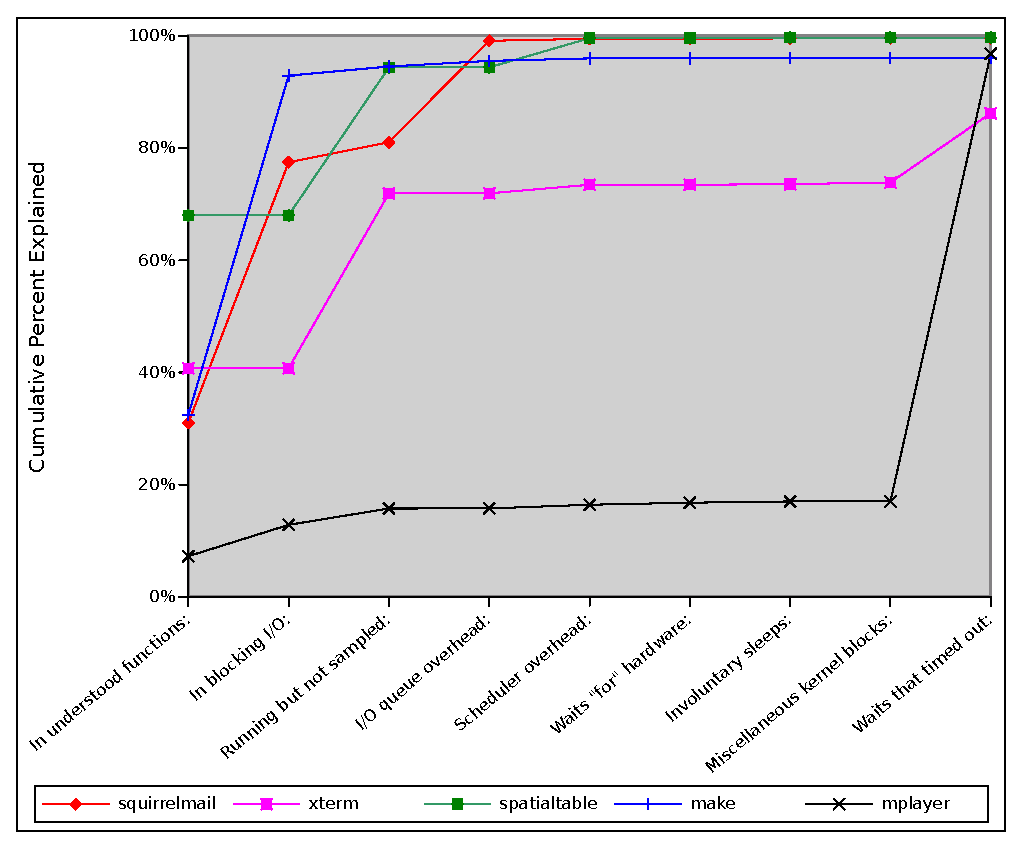
\includegraphics[width=3.2in]{images/5cumugraph}
\caption{Cumulative Percentage Explained}
\label{fig:resgraph}
\end{figure}

When one process invokes another and then goes to sleep, sometimes there is a delay between the first process going to sleep and the second running.  We describe this as ``scheduler overhead''.  Note that the opposite pattern is more common: often the next process begins running \emph{before} the previous process has departed.

\subsubsection{Waits ``for'' hardware}

These are waits which terminate with the receipt of an interrupt.  We place the word ``for'' in scare quotes because we have no visibility into that hardware.  Perhaps the hardware was working the entire time.  Or perhaps the interrupt reflects some external event.

\subsubsection{Involuntary sleeps}

These are waits do to pre-emption or interrupt handling.

\subsubsection{Miscellaneous kernel blocks}

There are various syscalls that block without blocking on anything we trace.  The most common of these is the kernel routine which moves processes from one CPU to another.

If this ever accounted for a large fraction of total time, it would suggest another case to be added to RSP.

\subsubsection{Waits that timed out}

These are waits that ended in timeout.  They can represent failed asynchronous operations, sleep statements, or other things.

In the MPlayer test case, they account for a large fraction of time.  More than half of this is MPlayer waiting until the correct time to display the next frame.

\subsubsection{Waiting on other path}

The organization of activity into control paths is not perfect.  For example, if a process sets another process going, then does some more work, and then waits for the child to complete, the child will be treated as a separate control path.  This means that after the work, the parent control path will be idle -- waiting on the child path.

Our ability to recognize this pattern is incomplete.  Much of the unaccounted time in the XTerm case is actually this.

This is displayed as time spent in our UI and in the table, but is subtracted from the denominator in constructing figure \ref{fig:resgraph}.

\subsection{Practical Results}

Producing lots of data is well and good, but can RSP produce information that useful to developers?  Here are three cases where it can.

\subsubsection{curl}

The first surprise looking at the Squirrelmail test case was a 5ms wait that timeout out in curl.  More measurements of curl alone demonstrated this was consistent: curl forks a worker thread for dns lookups and then polls slowly to see if it has finished.  No ordinary profiler would have detected this.  The code that actually ran was exactly correct.  Even the wait stack was reasonable.  And when the parent process finished waiting, the data it was waiting for was there.  The only problem was the child thread didn't write into the parent's poll.  Only by observing the mechanism by which the parent process exited the poll could this be detected.

Fixing the problem required only twenty lines of code, which took a few hours to write (for a programmer completely unfamiliar with the curl codebase).  All curl invocations are now almost 5ms faster.  The exact changes are shown in figure \ref{fig:curl}

The curl maintainers rejected the patch because it isn't compatible with Microsoft Windows, but at least their attention has been drawn to the problem.

\subsubsection{Squirrelmail}

Naively, one might think Squirrelmail's chain of operations was ``browser sends tcp to web server forks php interpreter sends tcp to imap server returns data''.  In fact, the php interpreter is built into apache (at least in our configuration) and the imap server (dovecot) is rather more complex.  It calls to two other programs: imap and imap-login, the latter of which calls a program called ``auth''.

In fact, auth is where roughly half of the time to produce the webpage is spent.  Of that, one third is spent in computation, mostly sha512, and the rest is spent syncing disks.

In is unlikely that anyone would guess that most of the time in reading an inbox was spent syncing disk as part of an authentication routine.  Nor can it be easily imagined that any other tool would allow us to discover this.  Furthermore, it seems likely (without looking at auth) that the syncs are unnecessary, and performance could be significantly improved.

A screenshot of the full visualization follows as figure \ref{fig:sq}

\subsubsection{SpatialTable}

In some ways, SpatialTable is the simplest of our test cases.  The number of processes is large, but the time is spent on the cpu and there is only one control path.  SpatialTable is also the only one of our test cases for which we were genuinely motivated to improve its performance.

SpatialTable's codebase contains many unnecessary data copies and other inefficient idioms.  RSP revealed that none of these mattered.  Instead of wasting time fixing them, the SpatialTable team concentrated exclusively on algorithmic optimizations.  With good reason it has been said that the important role of a profiler is not to help you optimize the 10\% of the code that needs it, but to help you \emph{not} optimize the 90\% that doesn't\cite{taoup}.  On this test, RSP is a great success.

\section{Future Work}

There are some specific features that would be useful:

\begin{itemize}
\item File names for disk I/O
\item Remote host and port pair for networking
\item Distinguish deliberate sleeps from other timeouts
\end{itemize}

As well as a few bugs still in the code.

At a higher level, a more thorough handling of the ``waiting on other path'' state would be valuable.  So would spreading across multiple nodes in a distributed system.

Also, the system would benefit from more robustness.  Dropped events in the perf log can leave RSP in a very confused state.  Also, while this does not happen often, a single wakeup from an unrelated process (perhaps because multiple requests to a server run into each other) can backchain into a lot of unrelated material in the trace.

Feature-wise, the system could handle work the process of interest kicks off and \emph{doesn't} wait for.  Also, it would be valuable to spread across multiple nodes and create a single integrated profile, matching incoming and outgoing network requests.


\section{Code}

All our code is available at \url{https://github.com/dspeyer/profiling}

\section{References}

\raggedright
\begin{thebibliography}{9}
\urlstyle{same}
\bibitem{perfwiki}
  \emph{Perf wiki}.
  \url{https://perf.wiki.kernel.org/index.php/Tutorial}

\bibitem{lttng}
  Desnoyers and Dagenais.
  \emph{The LTTng tracer: A low impact performance and behavior monitor for
  GNU/Linux}.
   In Linux Symposium.
   2006

\bibitem{lttngLwn}
  \emph{LTTng 2.0: Tracing for power users and developers}.
  2012.
  \url{http://lwn.net/Articles/491510/}

\bibitem{brendanGregg}
  Brendan Gregg.
  \emph{Brendan Gregg's blog}.
  \url{http://brendangregg.com/}

\bibitem{oncpu}
  Brendan Gregg.
  \emph{On-CPU Flame Graphs}.
   2014.
   \url{http://brendangregg.com/FlameGraphs/cpuflamegraphs.html}

\bibitem{offcpu}
  Brendan Gregg.
  \emph{Off-CPU Flame Graphs}.
   2014.
   \url{http://brendangregg.com/FlameGraphs/offcpuflamegraphs.html}

\bibitem{hotcold}
  Brendan Gregg.
  \emph{Hot/Cold Flame Graphs},
   2014.
   \url{http://brendangregg.com/FlameGraphs/hotcoldflamegraphs.html}

\bibitem{traceCompass}
  \emph{TraceCompass User Guide}.
  \url{http://archive.eclipse.org/tracecompass/doc/stable/org.eclipse.tracecompass.doc.user/User-Guide.html}

\bibitem{lbr}
  Ingo Molnar.
  \emph{perf updates for v4.1}.
  Linux Kernel Mailing List.
  2015.
  \url{https://lkml.org/lkml/2015/4/14/232}

\bibitem{Squirrelmail}
  \emph{Squirrelmail Documentation}.
  \url{http://squirrelmail.org/documentation/}

\bibitem{spatialtable}
  Speyer, Lee and Hu.
  \emph{SpatialTable: A Distributed Spatial Database}.
  Columbia Advanced Seminar on Distributed Systems.
  2015

\bibitem{bigtable}
  Chang et al.
  \emph{Bigtable: a distributed storage system for structured data}.
  OSDI.
  2006

\bibitem{pb}
  Kenton Varda.
  \emph{Protocol Buffers: Google's Data Interchange Format}.
  2008.
  \url{http://google-opensource.blogspot.com/2008/07/protocol-buffers-googles-data.html}

\bibitem{taoup}
  Eric Raymond.
  \emph{The Art of Unix Programming}.
  Addison Wesley.
  2003.
  \url{http://www.catb.org/esr/writings/taoup/html/}

\end{thebibliography}

\onecolumn
\newpage

\section{Appendix: Large Figures}

\vspace{1in}

\begin{figure}[h]
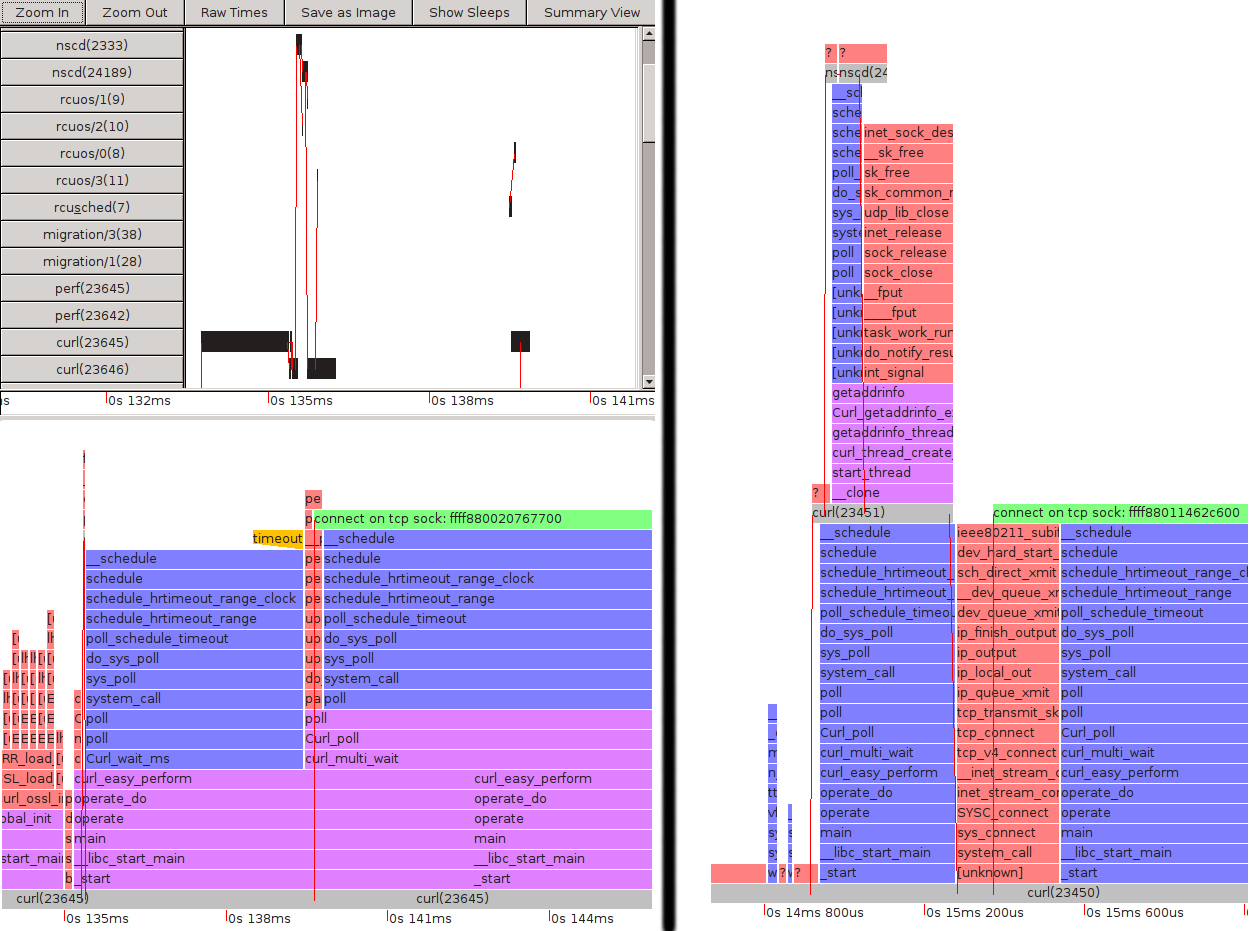
\includegraphics[width=6.5in]{images/curlBeforeAndAfter}
\caption{Curl DNS worker thread handling, before and after the fix}
\label{fig:curl}
\end{figure}

\begin{figure}[p]
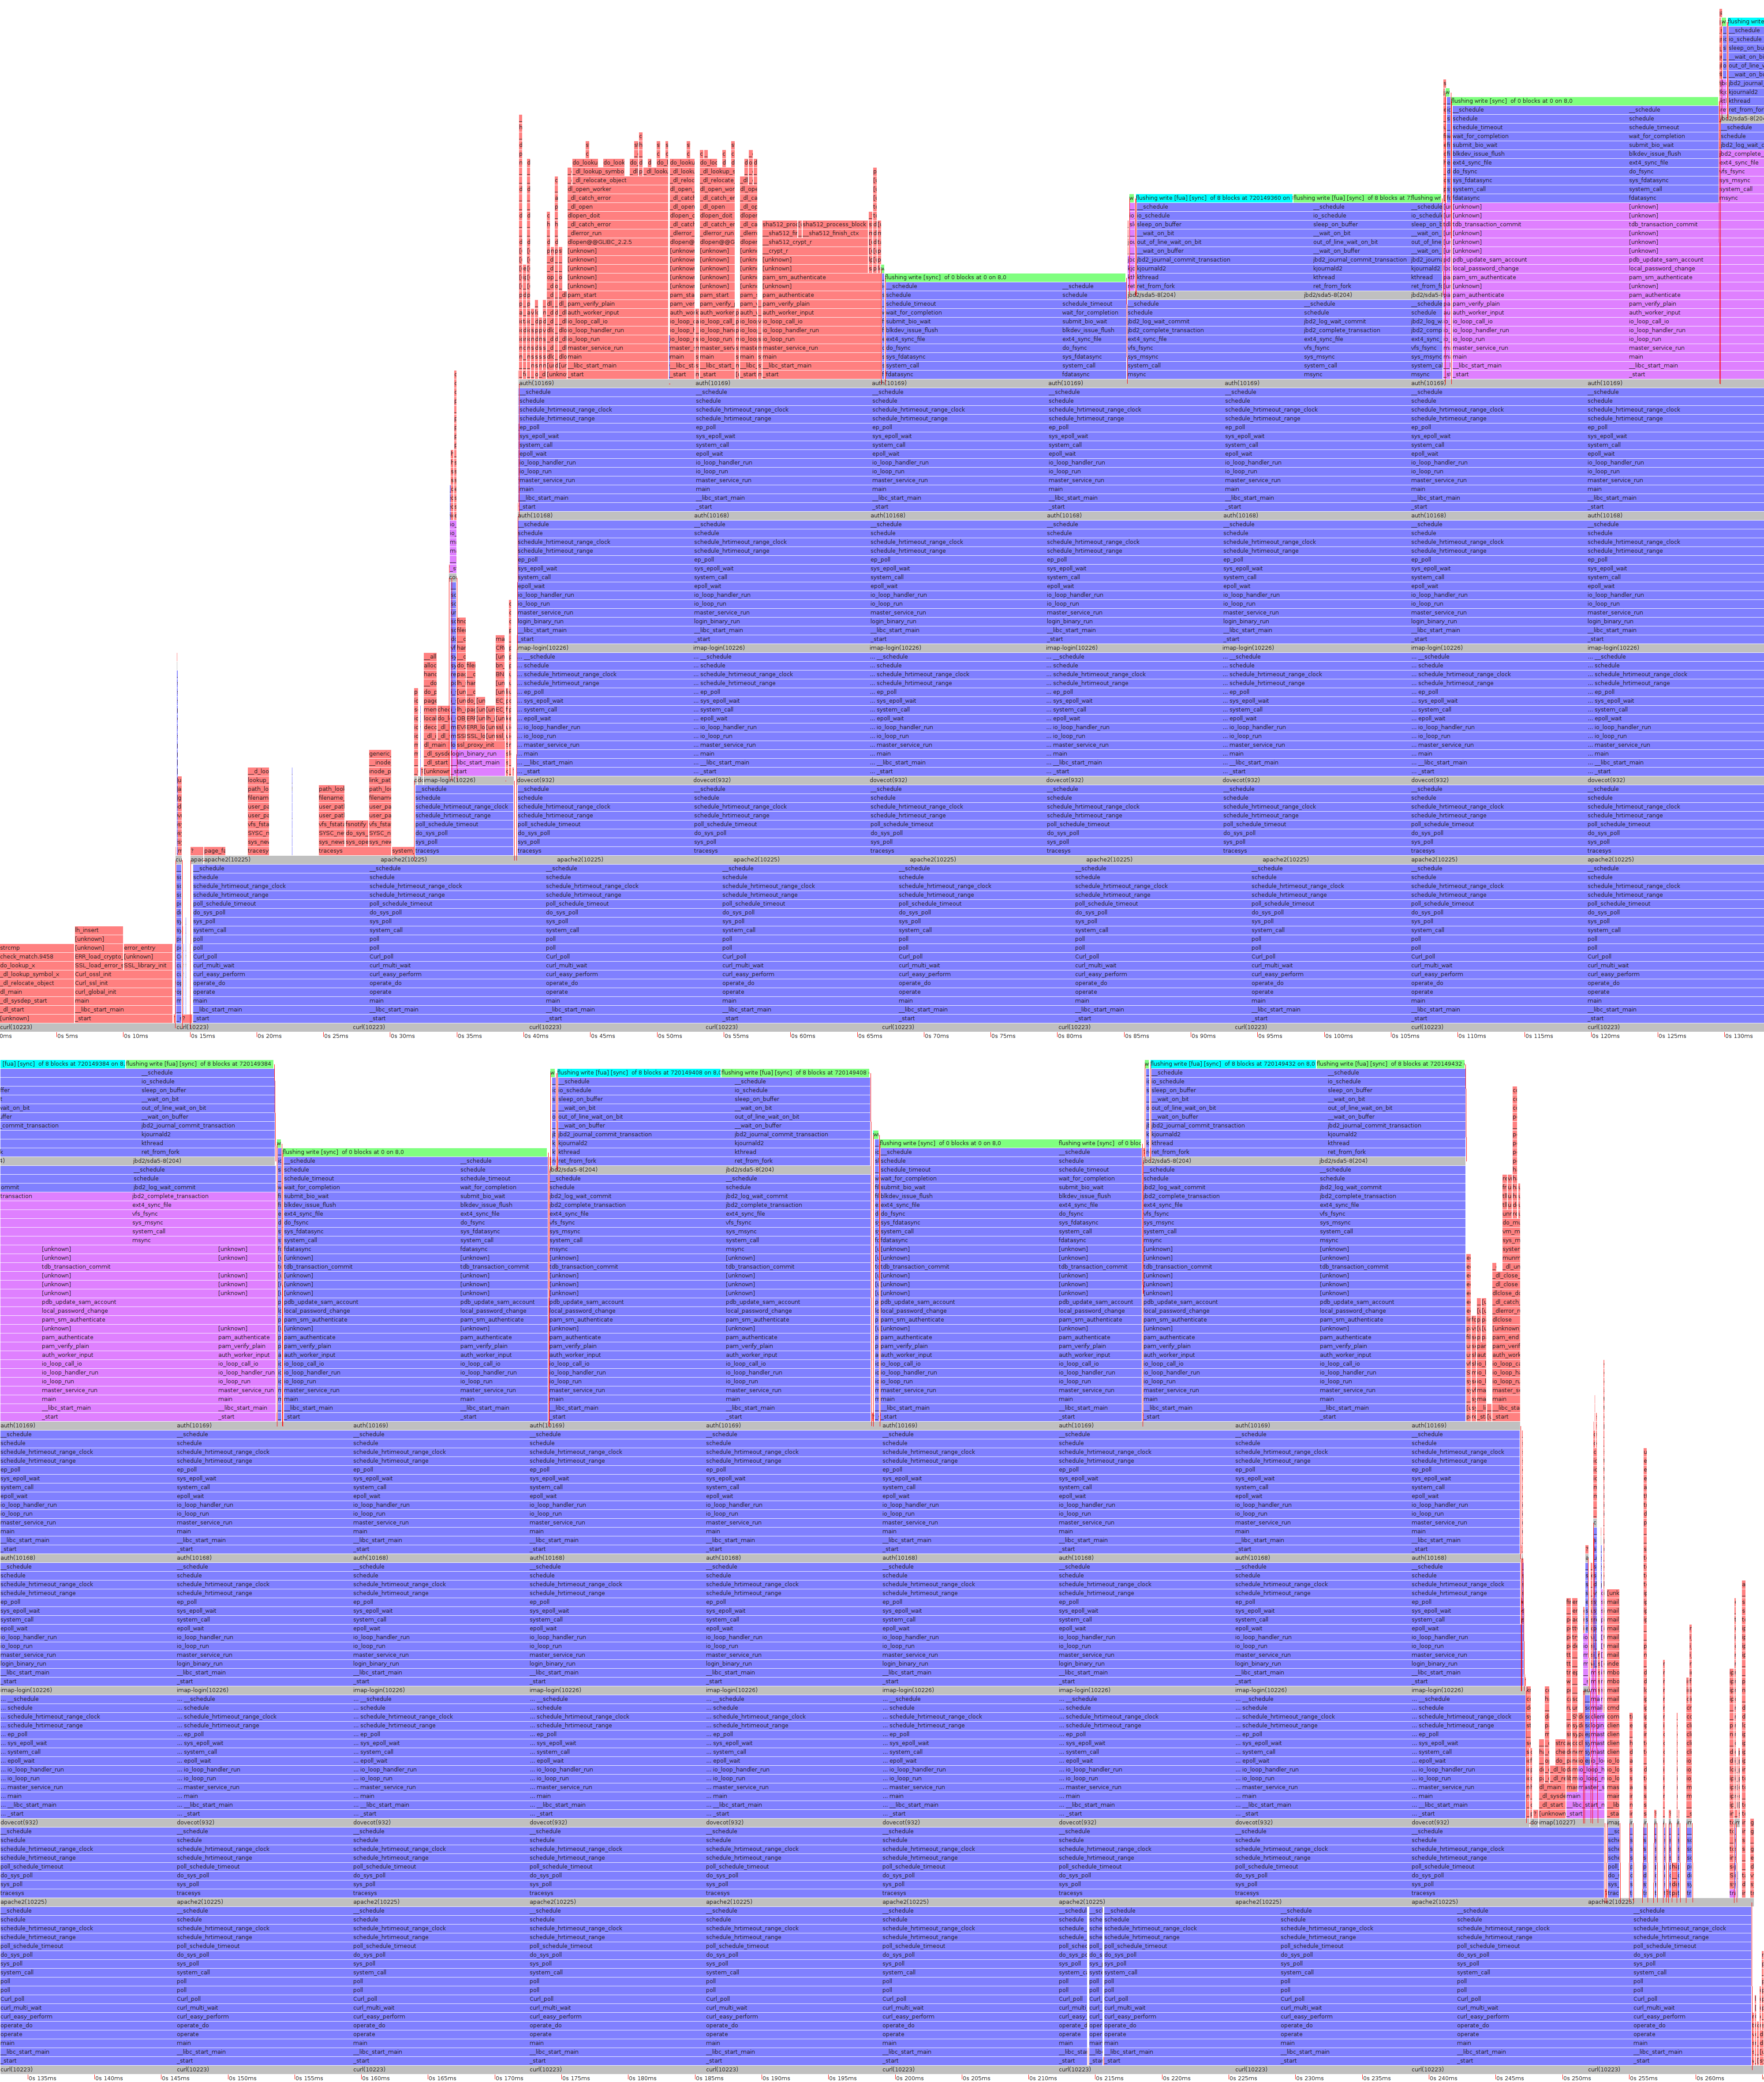
\includegraphics[width=6.5in]{images/squirrelbest}
\caption{The complete Squirrelmail flamegraph}
\label{fig:sq}
\end{figure}

\end{document}
